\documentclass[10pt,aspectratio=169]{beamer}  
\usetheme{CambridgeUS}

\usepackage{graphicx}
\usepackage{tikz}
\usetikzlibrary{shapes.geometric, arrows}
\usepackage{url}
\usepackage{etoolbox} % For \AtBeginEnvironment
\BeforeBeginEnvironment{flalign}{\setlength{\mathindent}{}}
\AfterEndEnvironment{flalign}{\setlength{\mathindent}{}}


% Redefine the section in toc and subsection in toc templates
\setbeamertemplate{section in toc}{\inserttocsectionnumber.~\inserttocsection}
\setbeamertemplate{subsection in toc}{\hspace{1.5em}\inserttocsectionnumber.\inserttocsubsectionnumber~\inserttocsubsection\par}

% Remove navigation symbols
\setbeamertemplate{navigation symbols}{}




\hypersetup{colorlinks,
    citecolor=blue,
    linkcolor=black,
    }
\addtobeamertemplate{navigation symbols}{}{%
    \usebeamerfont{footline}%
    \usebeamercolor[fg]{footline}%
    \hspace{1em}%

}

\mode<presentation>
{
  \usetheme{boxes}
}

\usepackage[english]{babel}
\usepackage{times}
\usepackage{tfrupee}
\usepackage[T1]{fontenc}
\usepackage{tabularx}
\usepackage{longtable}
\usepackage{hyperref,etoolbox}
\usepackage{url}
\usepackage{booktabs} 
\usepackage{tabularx}
\usepackage{multicol}
\usepackage{caption}
\usepackage{threeparttable}
\usepackage{tikz}
\usetikzlibrary{positioning, arrows.meta}
\usepackage[backend=biber, style=apa]{biblatex}

\addbibresource{ref.bib}



\newcommand{\fullpage}[1]{
  \begin{frame}
    \vfill
    {\Large #1}
    \vfill
  \end{frame}
}


\title{Assessing the Poverty Alleviating Effects of MSME
in India}
\author{Ishan Deodhar}
\vspace{0.8cm}
\institute{\normalsize {Under the guidance of \\ Mr. Balu Pawde, \\ Gokhale Institute of Politics and Economics}\vspace{0.8cm}}
\date{\today}


\begin{document}


\begin{frame}
  \titlepage
\end{frame}

\begin{frame}{Table of content}
    \tableofcontents 
\end{frame}

\section{Introduction}
\begin{frame}{Introduction}

{\fontsize{10pt}{12pt}\selectfont
    \begin{itemize}
        \item At independence, poverty was said to be alleviated through rapid industrialisation and large public works \parencite[ch. 1]{balakrishnan_indias_economy}.
        \item Poverty alleviation has been at the center of India's development agenda and We see poverty alleviation feature in multiple 5-year plans \parencite{kapila_indian_economy}.
        \item Poverty alleviation is the first on Sustainable Development Goals (SDG).
    \end{itemize}

\vspace{0.5cm}

    \begin{itemize}
        \item \textcite{amutha2022role} claims that MSMEs are the primary
        source of employment, production, exports, and GDP growth in India.
        \item MSMEs contribute to 29\% of India's GVA and 36\% of manufacturing output \parencite{MSME2023}.
        \item ``This sector (MSME) employs an estimated 59.7 million persons spread over 31 million enterprises. MSME sector accounts for about 45\% of the manufacturing output and around 40\% of the total export of the country" \parencite[739]{purakala2020role}.
        
        
    \end{itemize}
}
\end{frame}

\section{Literature Review}
\begin{frame}{Literature review}
    \fontsize{8pt}{10pt}\selectfont
        \renewcommand{\arraystretch}{1.2}
\begin{tabularx}{\textwidth}{lX}
    \toprule
    \textbf{Citation} & \textbf{Summary of findings} \\
    \midrule

    \parbox[t]{0.3\linewidth}{\textcite{harvie2003contribution} \& \textcite{Beck2003SMEGrowth} \& \textcite{MAKSIMOV2017244}} 
    & Study the effects of SME on poverty on a panel of countries. \textcite{harvie2003contribution} and \textcite{MAKSIMOV2017244} find SME to alleviate poverty in East Asian countries and low-income countries respectively, while \textcite{Beck2003SMEGrowth} use a panel of 75 countries and do not find any significant relationship between SME and poverty. \\
        & \\
    \parbox[t]{0.3\linewidth}{\textcite{nursini2020msmes}, \textcite{asikhia2016smes}, \textcite{abisuga2020smes}, \textcite{ali2014role} \& \textcite{manzoor2019role}} 
    & Find SME to have a negative effect on various Poverty measures in Indonesia, Nigeria, a Panel of Sub-Saharan countries, Pakistan, and a Panel of SAARC countries respectively. \\ 
        &  \\
    \parbox[t]{0.3\linewidth}{\textcite{vijayakumar2013empirical} and \textcite{manzoor2019role}} 
    & \textcite{vijayakumar2013empirical} and \textcite{manzoor2019role} find no effect of SME on poverty or economy in Sri Lanka and \textcite{manzoor2019role} don't find a significant effect of SME in Pakistan either. \\
     & \\
    \parbox[t]{0.3\linewidth}{\textcite{sinha2017study}, \textcite{manna2017status} \\ \& \textcite{manzoor2019role}} 
    & \textcite{sinha2017study} and \textcite{manna2017status} find that MSME  have grown substantially, with notable contributions to employment and GDP, specifically in the state of Chhattisgarh and Tamil Nadu, Uttar Pradesh, Gujarat, and West Bengal, respectively since the last MSME survey. \textcite{manzoor2019role} find SME to have poverty-alleviating effects in India.\\
    \bottomrule
\end{tabularx}
\end{frame}

\section{MSME growth and poverty}
\begin{frame}{MSME growth and poverty}

\vspace{0.5cm}    
    \fontsize{10pt}{12pt}\selectfont
    \begin{itemize}
\item The relationship between employment and poverty reduction could be attained on three conditions: (i) the overall growth rate of labour must be able to absorb new workers with high levels of productivity, (ii) job creation must produce an equitable job distribution between the poor and non-poor, and (iii) the jobs created must have a wage standard or at least a livable, satisfactory wage \parencite{singh1999role}.
\item When a high level of economic growth leads to increased production capacity and productivity, the poor have an opportunity to be absorbed into the various productive sectors that can generate higher incomes. Through this process, each labourer absorbed into these sectors would positively affect poverty alleviation \parencite{islam2004nexus}.
\item Thus, combining \textcite{islam2004nexus}, \textcite{singh1999role}, \textcite{MSME2023}, and \textcite{purakala2020role} MSME sector has a lot of potential in India to aid in poverty alleviation.
\end{itemize}
\end{frame}

\section{Research questions}
\begin{frame}{Research questions}

\fontsize{12pt}{12pt}
\begin{itemize}
    \item Does the number of MSME have an effect on poverty headcount in India?
    \item If yes, then-
    \vspace{0.3cm}
\setbeamerfont{itemize/enumerate subbody}{size=\fontsize{10pt}{17pt}}
    \begin{itemize}
    \item What is the nature and magnitude of the effect of the number of MSME on poverty?
    \item Does the enterprise level (Micro, Small, Medium) affect the magnitude and nature?
    \item Do the `grouped MSMEs' (Small-Medium and Micro-Small) have a different effect from each other on poverty?
    \end{itemize}
\end{itemize}  
\end{frame}

\section{Methodology}
\subsection{Data}
\begin{frame}{Methodology: Data}
    \fontsize{10pt}{12pt}\selectfont
    \begin{itemize}
        \item This study uses Annual Survey of Industries (ASI) data to identify the count of MSME in states of India.
    \item   Based on the gross value of plants and machinery assets, and \textcite{MinistryOfMSME2020}'s definition of MSME, this study classifies firms into Micro, Small, and Medium enterprises.
    \item \textbf{Micro}: $\leq Rs. 10$ million, \textbf{Small}: $\leq Rs. 100$ million, \textbf{Medium}: $\leq Rs. 500$ million.
    \vspace{0.5cm}
     \item This study uses CMIE's CPHS data for poverty estimations.
      \item  This study uses consumption-based poverty, using \textcite{rangarajan2014} i.e Rangarajan expert committee.
    \item The poverty threshold for urban hh. is MPCE of Rs. 1407 based on consumption of 2,155 kcal per person, per day; and for rural households is MPCE of Rs. 972 based on consumption of 2,090 kcal per person, per day \parencite{rangarajan2014}.   
    \item The expert Committee also imputes expenditure on clothing, rent, conveyance and education, rather than limiting the basket to only foods encompassing the normative nutrition levels \parencite{rangarajan2014}.
\end{itemize}
\end{frame}
\begin{frame}{Methodology: Computation of poverty headcount}
    \fontsize{10pt}{12pt}\selectfont
\begin{itemize}
    \item \textit{Total Expenditure} is used for classifying poverty. It is computed as the summation of all expenditures incurred by the household.
    \item Since Rangarajan committee's report was released in 2014, I adjust \textit{Total Expenditure} for inflation using CPI (consumer price index, headline inflation of India) to the base year 2014.
    \item From \textit{Total Expenditure}, variable $mpce_k$ is computed by dividing \textit{Total Expenditure} by \textit{Household Size}.
    \end{itemize}
    \vspace{0.5cm}
    \begin{itemize}
    \item \textcite{roy2022poverty} point out several biases in the instrument design of the CPHS, while comparing CPHS to NAS surveys. This study takes their suggestion to reweigh the adjusted weight.
    \item ``The non-response adjusted weight, by design, adds up to the Census’ population projections for a given year. We choose not to rely on these individual weights as due to the passage of time. Instead, we reconstruct individual level survey weights by multiplying household level weights and the household size for each round." \parencite[11]{roy2022poverty}.
        
    \end{itemize}
\end{frame}

\begin{frame}{Methodology: Computation of poverty headcount}

    \begin{multicols}{2}
Given that $k$ is rural.
    \[
    \textit{HH Poor}_{k} =
    \begin{cases}
        1 & \text{if } mpce_{K} \leq 972 \\
        0 & \text{otherwise}
    \end{cases}
    \]

    \columnbreak
Given that $k$ is urban.
    \[
    \textit{HH Poor}_{k} =
    \begin{cases}
        1 & \text{if } mpce_{K} \leq 1407 \\
        0 & \text{otherwise}
    \end{cases}
    \]
\end{multicols}

\begin{itemize}
    \item If we compute the average of \textit{HH Poor} since it takes values 0 or 1, we will get a proportion i.e. the headcount ratio.
\end{itemize}
\begin{equation} \nonumber
    P_i = \frac{\sum_{k=1}^{N} W_i \cdot \textit{HH poor}_{k}}{\sum_{k=1}^{N} W_i }
\end{equation} 

\normalsize
\begin{itemize}
    \item  Similarly, computing a weighted mean of the variable \textit{mpce} at state level will yield us the average MPCE of the state.
    \end{itemize}

\begin{equation} \nonumber
    MPCE_i = \frac{\sum_{k=1}^{N} W_i \cdot mpce_{k}}{\sum_{k=1}^{N} W_i}
\end{equation}

\end{frame}

\begin{frame}{Methodology: Control variables}
\begin{itemize}
    \item Real per capita GDP: I use real per capita state Gross domestic product (base as 2011) as a control for economic growth. Data is sourced from States of India, CMIE.
    \item Yeild per hectare: Higher levels of agriculture in a region could be a sign of under-development (in an economic sense) of the region. Incomes from agriculture are generally low compared and are often seasonal. Thus I use yield per hectare of foodgrains as a control. The data is sourced from States of India, CMIE.
    \item Urbanisation rate: Kundu (2007) posits that rural-urban migration can be a tool for poverty alleviation, the shift from casual employment to more stable forms of employment in urban areas has implications for poverty reduction. Thus, I control for urbanisation. The data on urbanisation (\%) per state comes from Census Technical Group's projections from the 2011 census.  
    \item Population: Population size has a direct impact on the need for social services, jobs, and resources—all of which are crucial components of poverty. Data is sourced from Census Technical Group's projections from the 2011 census. 
\end{itemize}
\end{frame}

\subsection{Summary statistics}

\begin{frame}{Summary statistics}
    \begin{table}[htbp]
    \small
    \centering
       \begin{tabular}{l*{5}{r}}
    \toprule
     Variable   &  Mean & Median & SD & Min & Max\\
     \midrule
      Poverty headcount (\%) & 13.38 & 9.65 & 12.55 & 0.011 & 65.7\\
      MPCE (Rs.) & 2437 & 2279 & 50.88 & 1002 & 5900 \\
      MSME & 3275 & 1946 & 3279.755 & 29 & 13284 \\
      Micro  & 807 & 525.8 & 738.771 & 9 & 3042 \\
      Small  & 1442.5 & 908.6  & 1404&  17  & 5649  \\
      Medium  & 1025.3 & 530.1 & 1196 & 3 & 5043  \\
      SGDP (Rs.) & 155236 & 140075 & 92450.85 & 29251 & 485645 \\
      Yield (per Hectare) & 5809 & 5588 & 1707.204 & 2157 & 10574 \\
      Urbanisation (\%) & 38.03 & 34.05 & 20.74 & 10.10 & 99.63 \\
      Population (`000) & 53929 & 36334 & 48992.73 & 664 & 224979 \\
      \bottomrule
    \end{tabular}
    \label{tab:sumstats}
\end{table} 

\end{frame}

\begin{frame}{Summary statistics}

\begin{itemize}
    \item Highest poverty, lowest MPCE: Odisha, 2014.
    \item Lowest poverty, highest MPCE: Goa, 2017.
    \item Highest MSME count: Maharashtra, 2019.
    \item Lowest MSME count: Tripura, 2019.
    \item Highest yield: Punjab, 2018.
    \item Lowest yield: Maharashtra, 2016.
    \item Highest urbanisation: Delhi, 2019.
    \item Lowest urbanisation: Himachal Pradesh, 2014.
    \item  The data contains a panel of 25 states and 6 time periods (2014-2019).
\end{itemize}
\end{frame}

\begin{frame}{Heatmap of MSME vs Poverty in India}
    \begin{minipage}{0.5\linewidth}
    \centering
    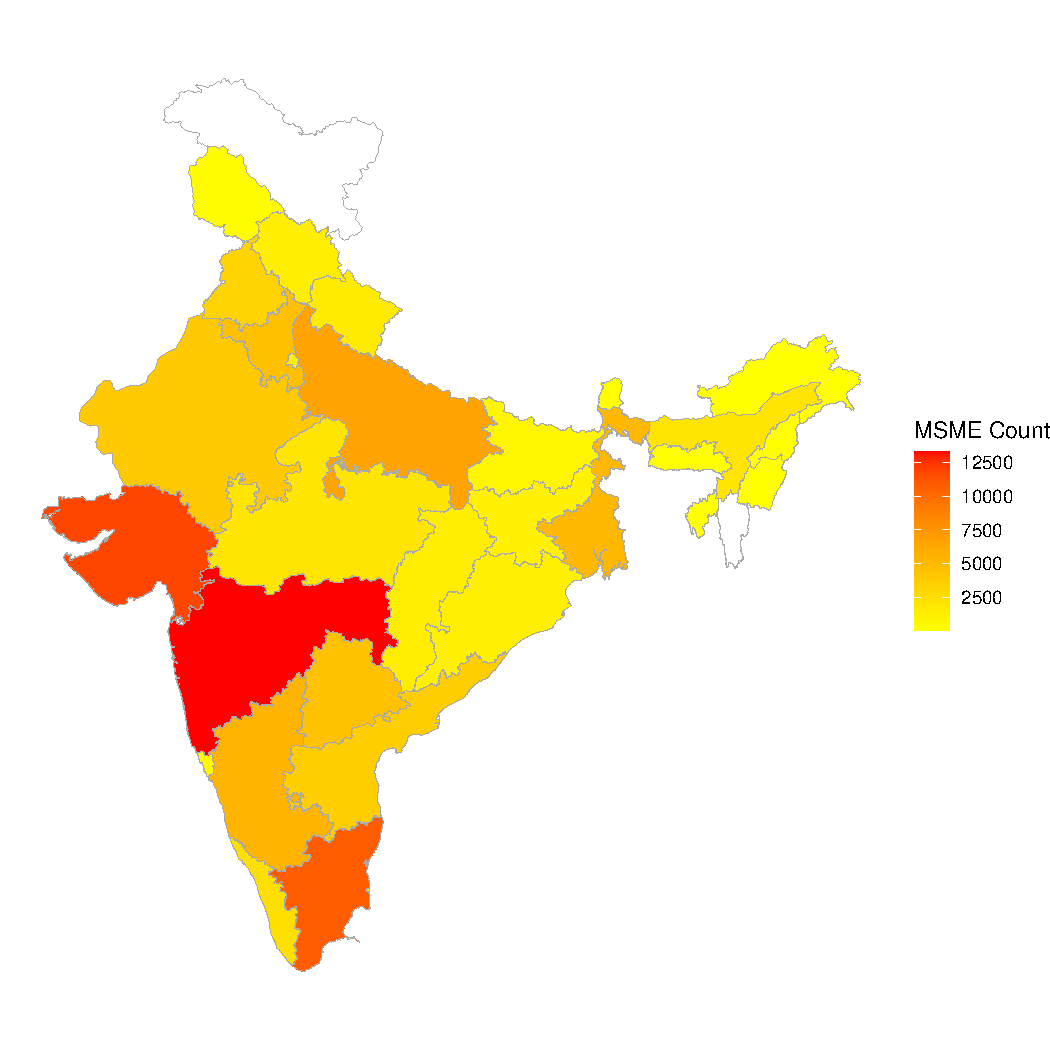
\includegraphics[width=\linewidth]{msme_plot.pdf}
  %  \caption{MSME in India}
    \label{fig:msme}
\end{minipage}%
\begin{minipage}{0.47\linewidth}
    \centering
    \includegraphics[width=\linewidth]{poverty_plot.pdf}
   % \caption{Poverty in India}
    \label{fig:poverty}
\end{minipage}
\end{frame}

\section{Econometric models}

\begin{frame}{Econometric models: Diagnostic tests}

\fontsize{10pt}{12pt}
\begin{itemize}

\item Hausman test is conducted to determine which model to use: random-effects or fixed-effects.
\item This study uses two-way fixed-effects models.
\item For model diagnostics: `Durbin-Watson' test- Autocorrelation, `Breusch-Pagan' test- Heteroscedasticity, and VIF- Multicollinearity.
\item Groupwise Heterscedasticity and Autocorrelation is detected.
\item  Robust Clustered Standard Errors are computed using Heteroscedasticity Consistent Covariance Matrix (HCCM) type HC3 \parencite{380055f1-819e-3149-a01c-cfab4e53c79f}.

\end{itemize}
\end{frame}

\begin{frame}{Econometric models: Equations}

\setlength{\jot}{8pt}
\begin{alignat}{2}
    P_{it} &= \beta_0 + \beta\ln{MSME_{it}} + \gamma\ln[Controls] + \epsilon \\
    MPCE_{it} &= \beta_0 + \beta MSME_{it} + \gamma[Controls] + \epsilon \\
    P_{it} &= \beta_0 + \beta_1\ln{Micro}_{it} + \beta_2\ln{Small}_{it} + \beta_3\ln{Medium}_{it} + \gamma\ln[Controls] + \epsilon \\
    MPCE_{it} &=  \beta_0 + \beta_1{Micro}_{it} + \beta_2{Small}_{it} + \beta_3{Medium}_{it} + \gamma[Controls] + \epsilon \\
    P_{it} &= \beta_0 + \beta_1\ln{MSE}_{it} + \beta_2\ln{Medium}_{it} + \gamma\ln[Controls] + \epsilon \\
    P_{it} &= \beta_0 + \beta_1\ln{SME}_{it} + \beta_2\ln{Micro}_{it} + \gamma\ln[Controls] + \epsilon 
\end{alignat}


  %  \end{equation}
\end{frame}

\section{Empirical results}

\begin{frame}{Empirical results}

\begin{table}[htbp]
    \centering
    \scriptsize
    \setlength{\tabcolsep}{4pt}
    \renewcommand{\arraystretch}{0.85} % Adjust inter-row spacing
    \begin{threeparttable}
        \begin{tabular}{lcccccc}
            \toprule
            \toprule
            & (1) & (2) & (3) & (4) & (5) & (6) \\
            Term & \(P\) & \(MPCE\) & \(P\) & \(MPCE\) & \(P\) & \(P\) \\
            \midrule
            \textit{MSME} & $-16.337^{*}$ & $-0.060$ & & & & \\
            & $(9.529)$ & $(0.058)$ & & & & \\
                   
            \textit{Micro} & & & $7.384$ & $0.037$ & & $6.657$ \\
            & & & $(4.710)$ & $(0.340)$ & & $(4.570)$ \\
                   
            \textit{Small} & & & $-21.685^{***}$ & $-0.648$ & & \\
            & & & $(7.644)$ & $(0.465)$ & & \\
                   
            \textit{Medium} & & & $-19.112^{**}$ & $0.417$ & $-22.836^{**}$ & \\
            & & & $(8.121)$ & $(0.276)$ & $(9.033)$ & \\
                    
            \textit{MSE} & & & & & $-4.760$ &  \\
            & & & & & $(8.199)$ &  \\
                 
            \textit{SME} & & & & & & $-37.647^{***}$ \\
            & & & & & & $(10.2412)$\\
                      
            \textit{SGDP} & $-17.775$ & $0.004^{***}$ & $-17.542$ & $0.003^{*}$ & $-11.187$ & $-20.097$ \\
            & $(19.167)$ & $(0.001)$ & $(14.547)$ & $(0.001)$ & $(17.761)$ & $(16.203)$ \\
                  
            \textit{Urban} & $2.680^{**}$ & $-65.451^{*}$ & $2.723^{***}$ & $-50.812$ & $2.589^{**}$ & $2.795^{***}$ \\
            & $(1.281)$ & $(38.667)$ & $(1.002)$ & $(40.534)$ & $(1.221)$ & $(1.044)$ \\
                   
            \textit{Yeild}  & $12.810$ & $0.100$ & $8.924$ & $0.099$ & $11.493$ & $ 9.416$ \\
            & $(9.042)$ & $(0.166)$ & $(8.031)$ & $(0.162)$ & $(8.486)$ &  $(8.103)$\\
            
            \textit{Population} & $223.283^{*}$ & $-0.000^{*}$ & $ 270.026^{**}$ & $-0.000$ & $259.609^{**}$ & $251.890^{**}$ \\
            & ($131.256$) & ($0.000$) & ($108.222$) & ($0.000$) & ($126.023$) & ($107.417$) \\
            
            \bottomrule
            Obs & 137 & 137 & 137 & 137 & 137 & 137 \\
            $R^{2}$ & 0.17 & 0.075 & 0.17 & 0.09 & 0.22 & 0.24 \\
            F-stat & 4.151 & 1.664 & 4.151 & 1.488 &  4.7129 & 5.363 \\
            P-value & $\leq 0.001$ & $0.149$ & $\leq 0.001$ & $0.179$ & $\leq 0.001$ & $\leq 0.001$ \\
            \bottomrule
            \bottomrule
        \end{tabular}        
    \begin{tablenotes}
        \item *** : $p\leq0.01$, ** : $p\leq0.05$, * : $p\leq0.1$
    \end{tablenotes}
    \end{threeparttable}
\end{table}
\end{frame}

\begin{frame} {Emirical results}
    \begin{itemize}
\item The coefficient for Micro and MSE is positive and statistically insignificant. 

\item A possible reason for Micro-enterprises not contributing to poverty-alleviation could be their limited capital. This lack of capital can lead to difficulties in expanding the business and may force these enterprises to use informal labour to save costs if it even employs people. 

\begin{itemize}
    \item Additionally, limited funds might mean using less advanced technology, resulting in lower productivity. 
    \item Consequently, Micro-enterprises might offer lower wages than Small and Medium enterprises. Together, these factors suggest that Micro-enterprises could unintentionally worsen poverty due to these inherent limitations and inefficiencies. 
\end{itemize}
     \end{itemize}
\begin{itemize}
    \item Small-Medium enterprises by definition have more capital than Micro, thus can operate at a bigger scale, use better technologies, and employ more people, possibly at better wage rates. Thus, SME have a poverty alleviating effect.
    \item When Micro enterprises expand, they evolve into Small enterprises. This progression is accompanied by an enhancement in the enterprise's capabilities, which can have positive implications for both employment opportunities and wage levels within the enterprise.
\end{itemize}

\end{frame}

\section{Conclusion}

\subsection{Limitations}
\subsection{Future scope of research}
\begin{frame}{Limitations}
    \fontsize{10pt}{12pt}\selectfont
\begin{itemize}
    \item \textcite{somanchi2021missing} refutes the claim of CPHS being nationally representative and claims that it underrepresents women and young children, overrepresents well-educated households, and underrepresents the poor.
    \item Trade or Service MSME are not factored in in this study. \textcite{kanitkar1994entrepreneurs} finds that only 19\%  of rural Micro-enterprises in his sample are involved in manufacturing, while higher proportion of Micro-enterprises are involved in services.
    \item  This study uses consumption-based poverty headcount as the main unit of analysis. Amartya Sen in ``Equality of what?"  argues on using MDP over any resource-based poverty measure. Due to time constraints and knowledge gaps, I am compelled to use a resource-based poverty measure. 
\end{itemize}   
    \vspace{0.5cm}
    \textbf{Future scope of research}
     \begin{itemize}
        \item Using a robust poverty measure like Multidimensional Poverty.
        \item Looking at poverty alleviation through labour absorption  and output of MSME.
        \item Linking productivity of MSME to wages, and its effect on Poverty.
    \end{itemize}
\end{frame}
\subsection{Conclusion}
\begin{frame}{Conclusion}
    \begin{itemize}
        \item Study concludes that the number of MSME has poverty-alleviating effects on the states of India.
        \item 1\% increase in the number of MSME, reduces poverty by 0.16 percentage points.
        \item Small and Medium enterprises have poverty-alleviating effects, whereas Micro has a more complicated relationship.
        \item Effect of Small and Medium enterprises at an individual level:
        \begin{itemize}
            \item 1\% increase in the number of Small ent. reduces poverty by 0.21 percentage points. 
            \item 1\% increase in the number of Medium ent. reduces poverty by 0.19 percentage points.  
        \end{itemize}
        \item MSE and SME have different effects on poverty.
        \item Effect of Small and Medium enterprises grouped together (SME): 1\% increase in the number of SMEs, reduces poverty by 0.37 percentage points.
    \end{itemize}


\end{frame}
\begin{frame}[c]{Feedback}
    \centering
    \vspace{0.5cm}
    \LARGE
    \textbf{Thoughts? Questions? Comments?}
    \vspace{0.5cm}

\end{frame}

\begin{frame}[allowframebreaks]{References}
\printbibliography%{ref}  Replace with your bibliography file name
\end{frame}
\end{document}
